\section{Opgaver}

\begin{opgave}{Hubbleloven}
    \opg Forklar hvorfor Hubbleloven kun gælder hvis $v>0$.
    \opg Kan Hubbleloven bruges til at bestemme afstande til himmellegemer, hvis lys er er blåforskudt?
\end{opgave}

\begin{opgave}{Den kritiske tæthed}
Den kritiske tæthed, $\rho_c$, kan defineres ud fra Friedmannligningen som den værdi af $\rho$, der opfylder ligning \eqref{friedmann} for et fladt univers.
\opg Hvilken værdi har $\kappa$ i et fladt univers?
\opg Vis at den kritiske tæthed er
%
\begin{align}
    \rho_c = \frac{1}{8\pi G}\left(3H^2 - \Lambda\right).
\end{align}
%
\opg Argumenter for at hvis $\Lambda \ll 3H^2$ så er
%
\begin{align} \label{eq:rho_c}
    \rho_c \simeq \frac{3H^2}{8\pi G}.
\end{align}
%
\opg Brug ligning \eqref{eq:rho_c} til at vise at den kritiske tæthed i Universet med den nuværende værdi af Hubbleparameteren, $H_0$, er
%
\begin{align*}
    \rho_\text{c} = \SI{8.6e-27}{\kilo\gram\per\cubic\metre}.
\end{align*}
\end{opgave}

\begin{opgave}{Et Univers af bolde}
Massetætheden i et univers kun bestående af bolde med massen $m_\mathrm{b} = \SI{1}{M_\odot}$ er
%
\begin{align} \label{eq:antalsdensitet}
    \rho = n_\mathrm{b}m_\mathrm{b},
\end{align}
%
hvor $n_\mathrm{b}$ er antalstætheden af bolde -- det vil sige antallet af bolde per volumen.
\opg Hvad skal antalstætheden af bolde være for at universet har den nuværende kritiske tæthed $\rho_\text{c} = \SI{8.6e-27}{\kilo\gram\per\cubic\metre}$?
\opg Den gennemsnitlige afstand mellem bolde i et sådant univers skalerer som $d_\mathrm{b} = n_\mathrm{b}^{-1/3}$. Bestem denne afstand.
\opg De fjerneste galakser vi kan se er i en afstand fra Jorden på $d_\mathrm{max} \approx \si{\clight}/H_0$. Bestem $d_\mathrm{max}/d_\mathrm{b}$.
\opg Er det sandsynligt at kunne se på den afstand vi kan, hvis vi levede i et univers af sådanne bolde? Advarsel: Denne opgave har intet facit, da radius af boldene ikke er oplyst. Men prøv gerne at opstille et generelt udtryk for sandsynligheden for at kunne se til afstand $s$, når man kigger i en tilfældig retning og boldene har radius $r$.

\opg Havde man brugt Mælkevejens masse, $m_\mathrm{b} = \SI{1e12}{M_\odot}$, ville man få $d_\mathrm{max}/d_\mathrm{b} = \SI{2.2e3}{}$, mens massen for en typisk galaksehob, $m_\mathrm{b} = \SI{1e15}{M_\odot}$, giver $d_\mathrm{max}/d_\mathrm{b} = \SI{2.2e2}{}$. Hvad fortæller disse udregninger os om Universet? Advarsel: Denne opgave har intet facit, da radius af boldene ikke er oplyst.
\end{opgave}

\begin{opgave}{Dopplerforskydning}%{2}
	Formlen for frekvensen ved Dopplerforskydning er
	\begin{align}
		f_{obs} = \frac{c+v_{obs}}{c+v_{kilde}} f_{kilde},
	\end{align}
	hvor $c$ er lydens hastighed i mediet, $f_{obs}$ er den observerede frekvens (udefra), $f_{kilde}$ er den udsendte frekvens, $v_{obs}$ er observatørens hastighed og $v_{kilde}$ er kildens hastighed.
	\opg En politibil kører mod dig 30 meter væk, men er 20 meter fra centrum af vejen når du kigger ligeud (se skitsen på Figur \ref{politi}). Tegn hastighedsvektoren og hastighedskomponenterne der peger henholdsvis parallelt med din synsvinkel og vinkelret på den. 
	\opg Bilens speedometer viser, at den kører 50 km/t. Brug trigonometri til at beregne hvor stor en hastighedskomponent, der peger mod dig (radiel hastighed). Skitsér groft en graf over radiel hastighed som funktion af tid og antag, at bilens hastighed er konstant.
	\opg Politibilens sirene udsender lyd med en frekvens på 800 Hz. Du står stille, og det er en let kølig dag med 15 grader, hvor lydens fart i luft er 340 m/s. Ved hvilken frekvens hører du tonen?
	\begin{figure}[h!]
		\centering
		\includegraphics[width=0.5\textwidth]{opg/figurer/Politi.png}
		\caption{}
		\label{politi}
	\end{figure}
\end{opgave}

\begin{opgave}{Skalafaktor}%{1}
	Temperaturen af den kosmiske mikrobølgebaggrund er i dag 2.73 K. Strålingen blev udsendt ved "rekombinationen", hvor universet var koldt nok til at elektroner kunne binde sig til atomkernerne. Det var en mindre exciteret tilstand, så atomerne udsendte energi som fotoner. Man kan måle, at det har krævet en temperatur på kun 3000 K. Brug at temperaturen udviklede sig som
	\begin{align}
		T(t)=\frac{T_0}{a(t)}
	\end{align}
	til at finde ud af, ved hvilken rødforskydning rekombinationen fandt sted.
\end{opgave}

\begin{opgave}{Rødforskydning af kvasar}%{1}
	Kvasarer (eng:”quasars” fra ”quasi-stellar radio sources”) er de mest energirige og
	fjerne medlemmer af objekterne kendt som aktive galaksekerner (eng:”AGN: Active
	Galactic Nuclei”). Kvasarer har siden deres opdagelse været omgivet af mystik, men
	der er nu opnået generel enighed om, at de er kompakte regioner i massive galakser,
	der indeholder det centrale supermassive sorte hul. De kæmpe mængder energi der
	bliver udstrålet af kvasarerne stammer fra al stoffet, som falder ind mod det sorte
	hul og bliver slynget ud.
	Et kvasar-spektrum er vist i Figur \ref{kvasar}.
	\\
	I Balmer-serien hopper en elektron til 2. orbital fra en mere exciteret tilstand. Den første af disse kaldes H-$\alpha$ og er faldet fra orbital 3 til 2. Den næste er H-$beta$ fra orbital 4 til 2 osv. Fotoner, der udsendes ved H-$\alpha$-overgangen, har en bølgelængde på 656 nm. Ofte måler man i ångstrøm (Å) som er $10^{-10}$ m.\\
	%Aflæs bølgelængden for H-$\beta$ på Figur \ref{spektrum} og beregn rødforskydningen.
		\begin{figure}[h!]
			\centering
			\includegraphics[width=0.5\textwidth]{opg/figurer/kvasarkunst.jpg}
			\caption{En kunstnerisk forestilling af en kvasar. Kilde: \cite{NASA_ESA_quasar}} %https://pbs.twimg.com/profile_images/683524276058763264/xyAc-NvD.jpg
			\label{kvasarkunst}
		\end{figure}
	\begin{figure}[h!]
		\centering
		\includegraphics[width=0.5\textwidth]{opg/figurer/kvasar.png}
		\caption{Spektrum af kvasaren 3C273. Kilde: \cite{YatesGardenQuasarSpectrum}} %http://www.astrosurf.com/buil/us/spe6/qso1.gif
		\label{kvasar}
	\end{figure}
	\opg Ud fra din viden om H-$\alpha$-overgangen, bevæger kvasaren sig så mod eller væk fra os?
	\opg Hvad er kvasarens radielle hastighed?
	\opg Man ser tit, at spektrallinjerne fra kvasarer er meget brede, fordi gassen bevæger sig hurtigt omkring det sorte hul, hvilket giver en Doppler-forbredning
	(lyset bliver både rød- og blåforskudt). Estimér bredden af H-$\alpha$-linjen, $\Delta\lambda_{obs}$, og udregn gassens fart ved 
	\begin{align}
		v_{gas}=\frac{\Delta \lambda_{obs}}{2\lambda_{0}}c
	\end{align}
\end{opgave}

\begin{opgave}{Afstande} %{3}
	\\  		
	\begin{figure}[h!]
			\centering
			\includegraphics[width=0.5\textwidth]{opg/figurer/ComovingDistance.png}
			\caption{Kilde: \cite{vardanyanICosmosCosmologyCalculator}.} %http://www.icosmos.co.uk/index.html
			\label{comoving} 
		\end{figure}
	\opg Opskriv luminositetsafstanden $D_L$ som funktion af vinkelafstanden $D_A$.
	\opg I et fladt univers er $D_M=D_C$. $D_C$ kaldes comoving distance, og med $\Omega_m=0.3$ og $\Omega_{\Lambda}=0.7$ opfører det sig som plottet på Figur \ref{comoving}. 
	Hvor stor er $D_L$ og $D_A$ ved $z=1$? \\
	Hvad med ved $z=9$? Giver ændringerne mening?
	\opg Hvor stor er den radielle hastighed for et objekt med $z=10$? Oplys svaret som procent af lysets fart i vakuum. Dengang var universet for resten kun  478 mio. år gammelt.
\end{opgave}

\begin{opgave}{Andromeda-galaksen}
		\begin{figure}[h!]
			\centering
			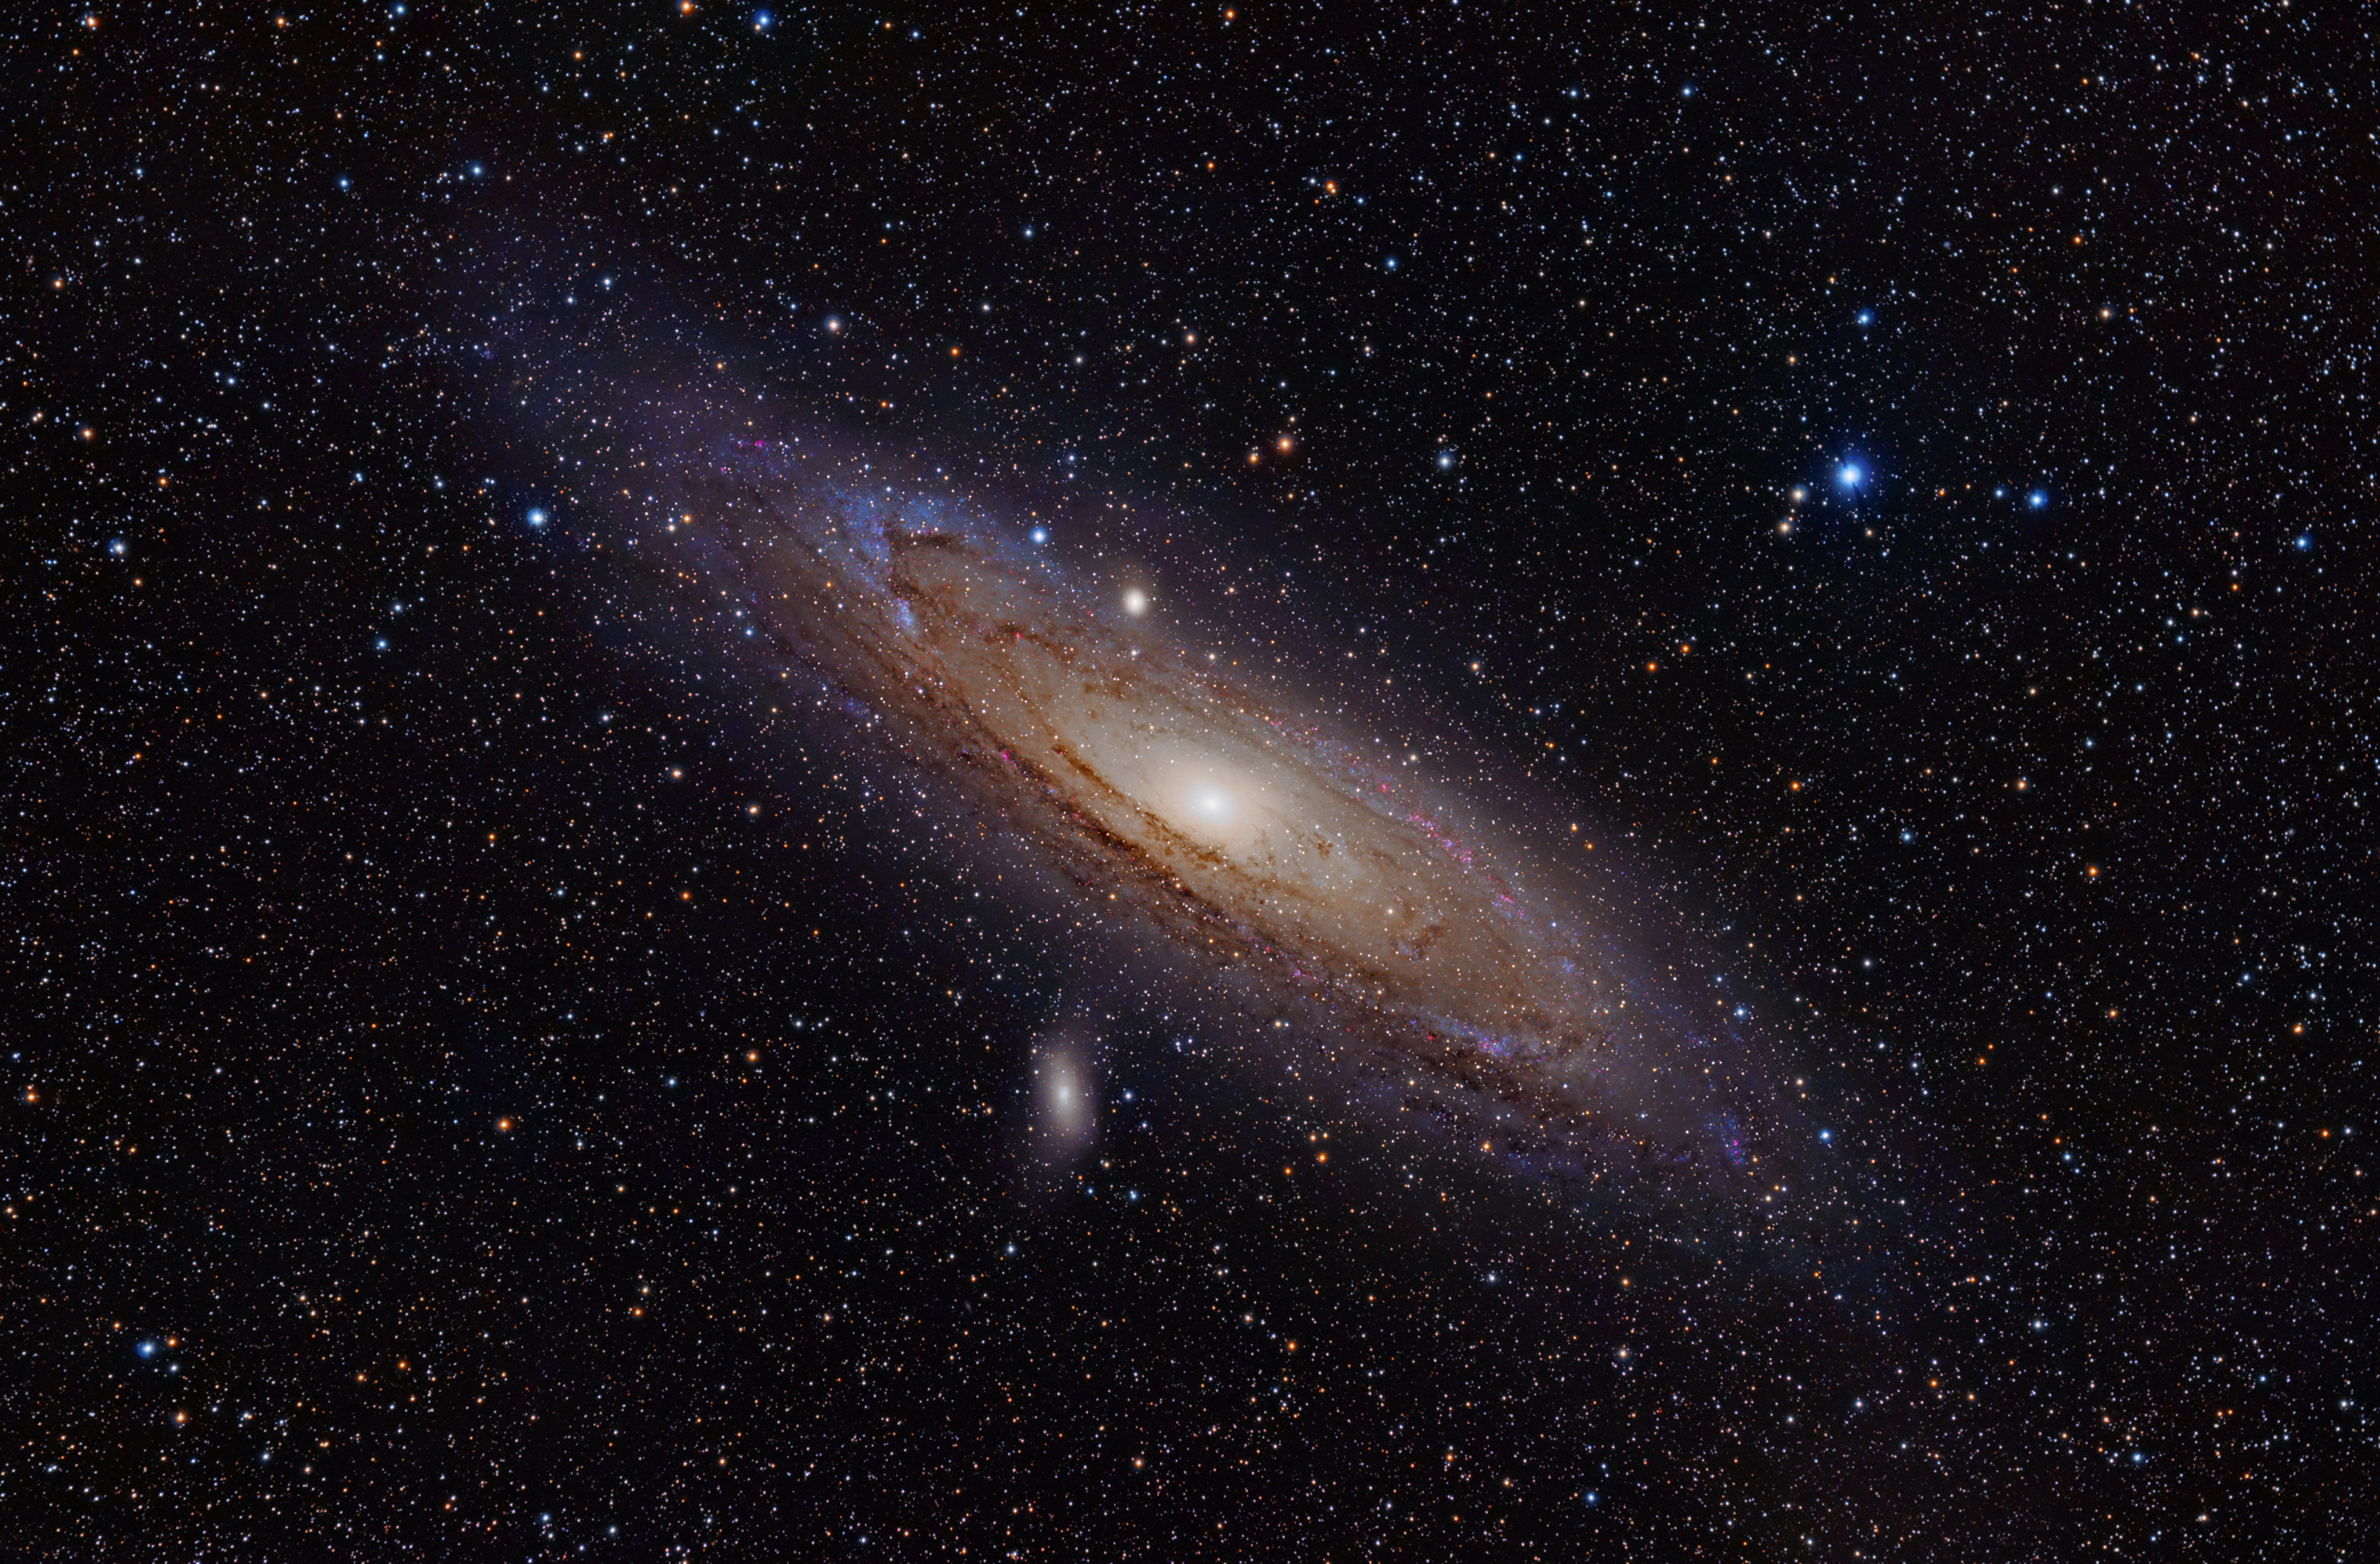
\includegraphics[width=0.5\textwidth]{opg/figurer/andromeda.jpg}
			\caption{Kilde: \cite{AndromedaGalaxy2019}.} %https://upload.wikimedia.org/wikipedia/commons/9/98/Andromeda_Galaxy_%28with_h-alpha%29.jpg
			\label{andromeda} 
		\end{figure}\\
	Andromeda-galaksen eller Messier-31 (M31) er den nærmeste spiralgalakse, og den største galakse i den Lokale Gruppe, som er en samling af ca. 50 galakser, heriblandt vores egen, Mælkevejen.  
	\opg Det observerede lys fra Andromeda har en rødforskyning på $z = -0.001$.
	%\opg Det observerede lys fra Andromeda har en rødforskydning på $z = −0.001$.
	Hvad er Hubbleafstanden til galaksen, fundet ved hjælp af Hubbles lov? Antag Hubblekonstanten er $H_0=70 km s^{-1} Mpc^{-1}$.
	\opg Gennem andre metoder har man fundet afstanden til 2,5 mio. lysår. Hvornår støder Andromeda og Mælkevejen sammen? Hvad tror du, det kommer til at betyde? Antag hastigheden er konstant, og Andromeda har direkte kurs mod os.
\end{opgave}




%\chapter{Astrofysik Facitliste}
%\section*{Astrofysik}
